\chapter{Detekcia objektov v obraze}

    Pre niektoré techniky klasifikácie objektov je nutné najprv v obraze tieto objekty nájsť. Existuje k tomu veľké množstvo metodík, pri čom každá z nich má svoje výhody a nevýody. Je teda nutnosťou zistiť ktorá metóda najviac vyhovuje použitiu pre túto prácu.

\section{Prahovanie}

    Prahovanie je jasová transformácia pri ktorej je šedotónový obraz rozdelený na dve a viac oblastí podľa jasovej úrovne pixelov. O tom, do ktorej z oblastí je daný pixel priradený rozhoduje prah, ktorého hodnotu je treba určiť. Výsledkom je obraz s len dvomi úrovňami jasu - binárny obraz.

    Pri správnom predspracovaní obrazu prahovaním, je možné v ňom jednoducho oddeliť objekty od pozadia, v prípade ak sa jas objektu dostatočne lýši od jasu pozadia. Ak sa však jasové hodnoty objektu a pozadia príliš podobajú, nemusí existovať dostatočne robustné určenie prahu oddeľujúceho objekty od pozadia.

    \begin{figure}[!ht]
        \begin{center}
            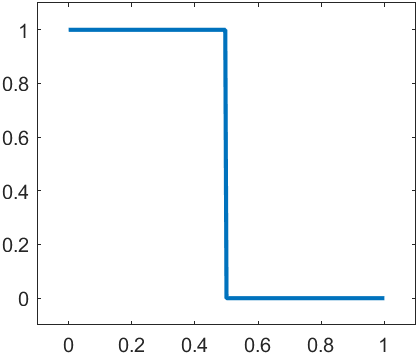
\includegraphics[scale=.4]{obrazky/threshold/thresholding.png}
        \end{center}
        \caption{Funkcia prahovania s prahom 0.5 pre svetlé pozadie}
    \end{figure}

\subsection{Globálne prahovanie}

    Globálne prahovanie je často používaná technika pri ktorej je použítý jediný prah na celý obraz, čo nemusí byť vhodné v prípade ak je jasová úroveň pozadia rôzna v rôznych miestach obrazu.

    \begin{itemize}
        \item \textbf{Jednoduché prahovanie} je technika pri ktorej je globálny prah určený dopredu ručne. V prípade že sa jasová úroveň pozadia v čase mení, je vhodnejšie použiť techniky s adaptívnym nastavením prahu.

        \item Prahovanie \textbf{podľa známeho rozloženia} predpokladá že poznáme relatívnu veľkosť oblasti ktorú zaberá pozadie v obraze. Ak vieme že objekt je svetlejší ako pozadie, môžeme určiť prah z kumulatívneho histogramu tak, aby relatívny počet pixelov pod úrovňou prahu bol rovnaký ako oblasť ktorú ma zaberať pozadie.

        \item Algoritmus \textbf{K-Means} (K priemerov) pre zhlukovú analýzu, rozdeľuje dáta do skupín s cieľom minimalizovať vzdialenosť bodov v zhluku a maximalizovať vzdialenosť medzi zhlukmi. Jedná sa o algorytmus učenia bez učiteľa. Funguje na princípe iterovaného posúvania \emph{k} stredov zhlukov (v prípade binárneho prahovania je \emph{k = 2}), smerom k priemeru hodnôt priradenému danému stredu v aktuálnom kroku.

        \item \textbf{Otsuova metóda} automatického určenia prahu je založená na maximalizovaní vzájomnej odchýlky medzi triedami. Využíva normalizovaný kumulatívny histogram z ktorého určuje vzájomnú rozptyl pre všetky možné hodnoty prahu a vyberá ten optimálny. 
    \end{itemize}

    \begin{figure}[!ht]
        \centering
        \begin{tikzpicture}[>=stealth, node distance=5cm]
            \node (image1) {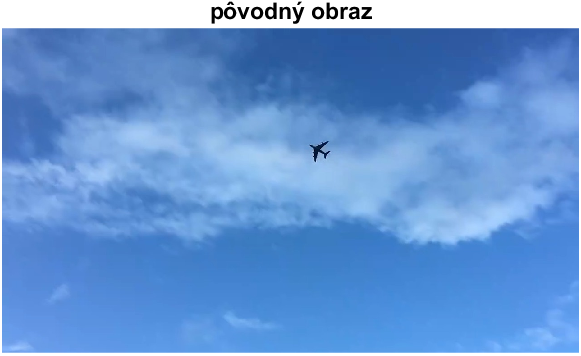
\includegraphics[width=.3\textwidth]{obrazky/threshold/img.png}};
            \node (image2) [right of=image1] {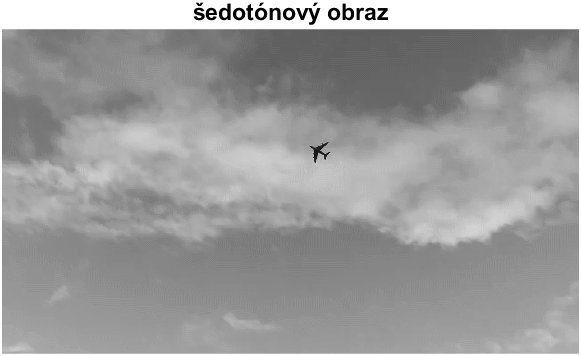
\includegraphics[width=.3\textwidth]{obrazky/threshold/img_gray.png}};
            \node (image3) [right of=image2] {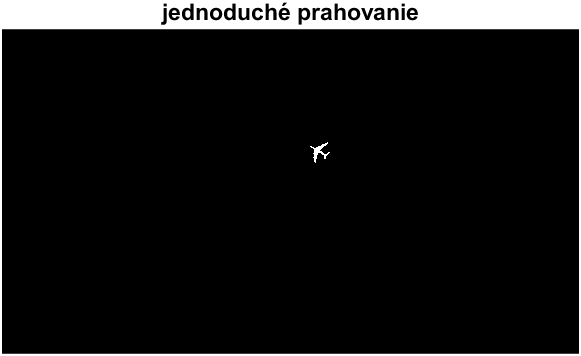
\includegraphics[width=.3\textwidth]{obrazky/threshold/img_simple_thresh.png}};

            \draw[->] (image1) -- (image2) node[midway, above] {};
            \draw[->] (image2) -- (image3) node[midway, above] {};
        \end{tikzpicture}
        \begin{tikzpicture}[>=stealth, node distance=5cm]
            \node (image1) {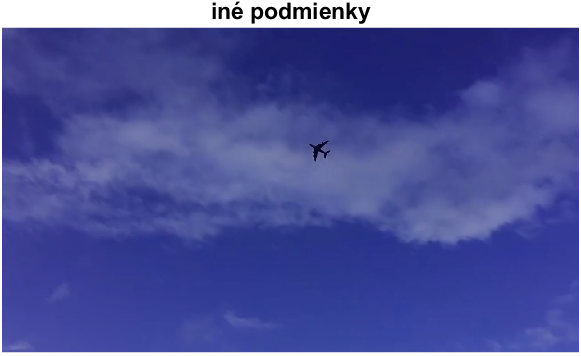
\includegraphics[width=.3\textwidth]{obrazky/threshold/img_dark.png}};
            \node (image2) [right of=image1] {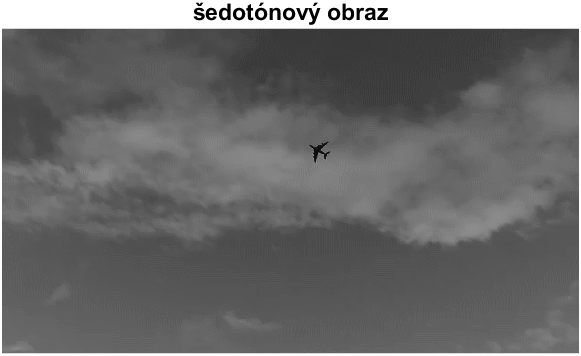
\includegraphics[width=.3\textwidth]{obrazky/threshold/img_dark_gray.png}};
            \node (image3) [right of=image2] {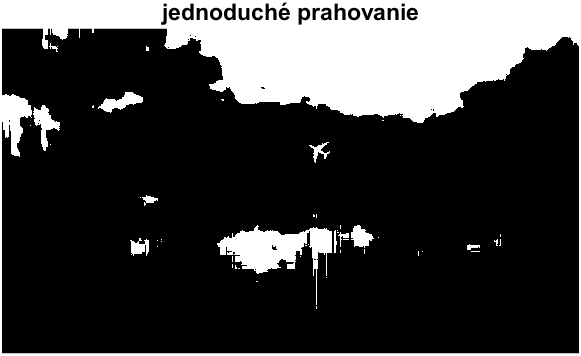
\includegraphics[width=.3\textwidth]{obrazky/threshold/img_dark_simple_thresh.png}};

            \draw[->] (image1) -- (image2) node[midway, above] {};
            \draw[->] (image2) -- (image3) node[midway, above] {};
        \end{tikzpicture}
        \caption{Jednoduché prahovanie}
    \end{figure}

    \begin{figure}[!ht]
        \centering
        \begin{tikzpicture}[>=stealth, node distance=5cm]
            \node (image1) {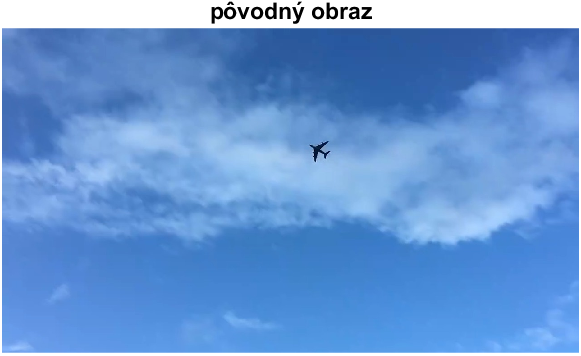
\includegraphics[width=.3\textwidth]{obrazky/threshold/img.png}};
            \node (image2) [right of=image1] {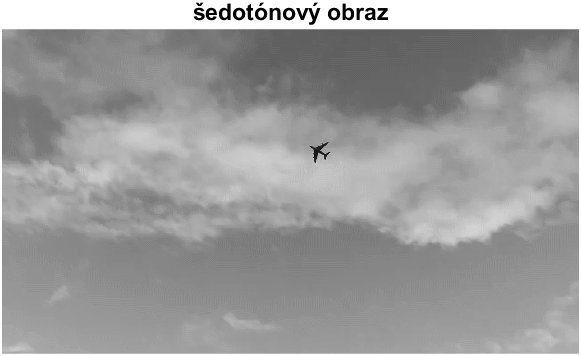
\includegraphics[width=.3\textwidth]{obrazky/threshold/img_gray.png}};
            \node (image3) [right of=image2] {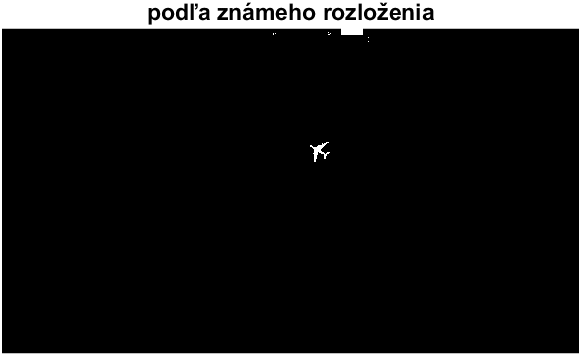
\includegraphics[width=.3\textwidth]{obrazky/threshold/img_thresh_distr.png}};

            \draw[->] (image1) -- (image2) node[midway, above] {};
            \draw[->] (image2) -- (image3) node[midway, above] {};
        \end{tikzpicture}
        \begin{tikzpicture}[>=stealth, node distance=5cm]
            \node (image1) {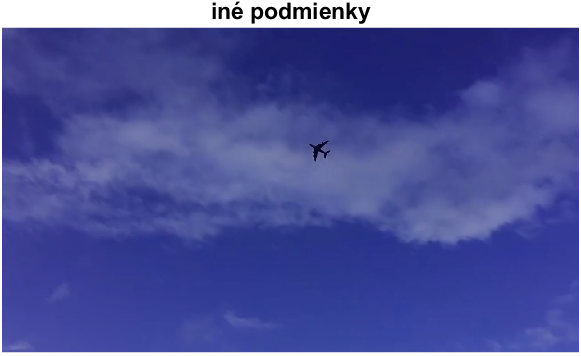
\includegraphics[width=.3\textwidth]{obrazky/threshold/img_dark.png}};
            \node (image2) [right of=image1] {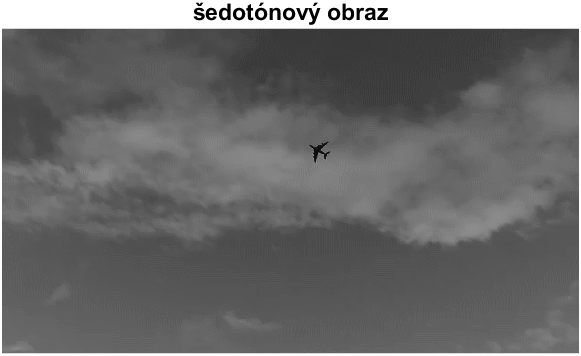
\includegraphics[width=.3\textwidth]{obrazky/threshold/img_dark_gray.png}};
            \node (image3) [right of=image2] {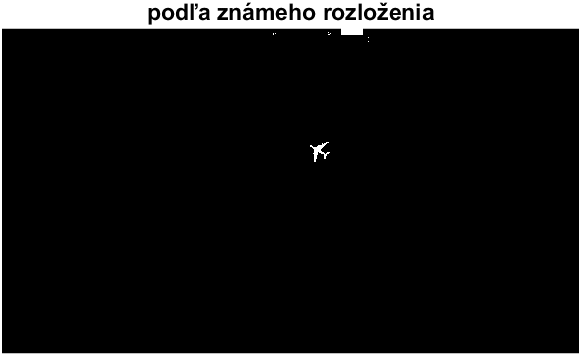
\includegraphics[width=.3\textwidth]{obrazky/threshold/img_thresh_distr.png}};

            \draw[->] (image1) -- (image2) node[midway, above] {};
            \draw[->] (image2) -- (image3) node[midway, above] {};
        \end{tikzpicture}
        \caption{Automatické prahovanie (podľa známeho rozloženia)}
    \end{figure}

\subsection{Lokálne prahovanie}

    V prípade že je jas pozadia rôzny v rôznych častiač obrazu, je vhodné určiť hodnotu prahu z jasovej úrovne okolia každého prahovaného pixelu. Toto takzvané adaptívne prahovanie, má síce vyžšiu výpočetnú náročnosť ako jednoduchšie globálne prahovanie, keďže je nutné určiť prah pre každý bod obrazu samostatne, je však robustnejšie voči nevhodnému pozadiu.

    \begin{figure}[!ht]
        \centering
        \begin{tikzpicture}[>=stealth, node distance=5cm]
            \node (image1) {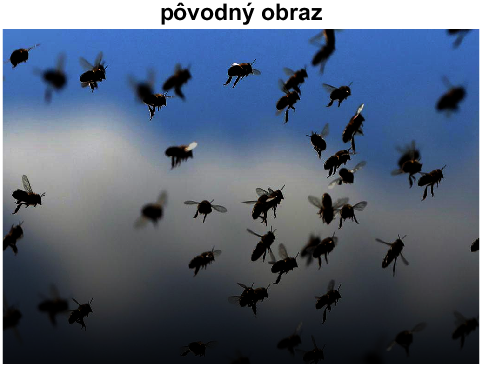
\includegraphics[width=.3\textwidth]{obrazky/threshold/img2.png}};
            \node (image2) [below of=image1] {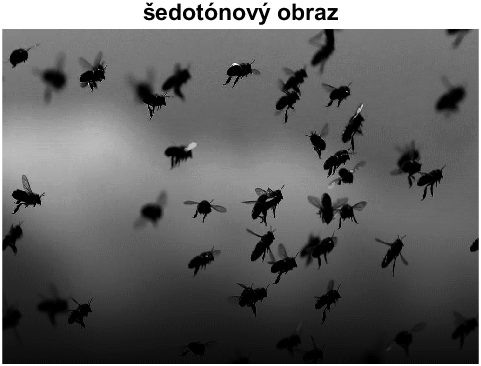
\includegraphics[width=.3\textwidth]{obrazky/threshold/img2_gray.png}};
            \node (image3) [left of=image2] {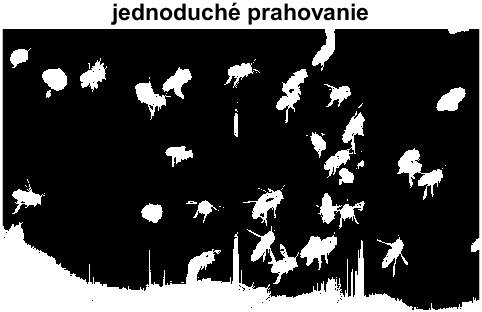
\includegraphics[width=.3\textwidth]{obrazky/threshold/img2_simple_thresh.png}};
            \node (image4) [right of=image2] {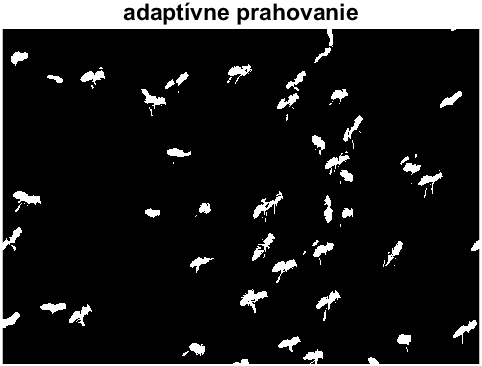
\includegraphics[width=.3\textwidth]{obrazky/threshold/img2_adaptive_thresh.png}};

            \draw[->] (image1) -- (image2) node[midway, above] {};
            \draw[->] (image2) -- (image3) node[midway, above] {};
            \draw[->] (image2) -- (image4) node[midway, above] {};
        \end{tikzpicture}
        \caption{Adaptívne prahovanie (podľa známeho rozloženia)}
    \end{figure}

\section{Detekcia hrán}

    Ako jednu z metód vyhľadávania objektov v obraze je možné využiť obraz hrán a vyhľadať v ňom kontúry objektov. Opäť existuje niekoľko spôsobov ako získať obraz hrán a ako ho využiť k segmentácii obrazu, teda k detekcii objektov.

    Na vytvorenie obrazu hrán z nasnímaného obrazu sa používa konvolúcia obrazu s operátorom navrhnutým tak aby aproximovalo deriváciu určitého rádu. Medzi často používané operátory patria Prewittov a Sobelov operátor, ktoré aproximujú prvú deriváciu v určitom smere (horizontálnom, vertikálnom, diagonálne). Druhú deriváciu aproximuje Laplaceov operátor, používa sa tiež v kombinácii s Gaussovým filtrom (LoG operátor), čo má za následok zníženie citlivosti na šum.

    % konvolučné operátory - hranové detektory
    \begin{figure}[!ht]
        \centering

        \begin{minipage}[b]{0.2\textwidth}
            \[
                \begin{bmatrix}
                    -1 & 0 & 1 \\
                    -1 & 0 & 1 \\
                    -1 & 0 & 1 \\
                \end{bmatrix}
            \]
            \centering
            Prewittov operátor
        \end{minipage}
        %
        \begin{minipage}[b]{0.2\textwidth}
            \[
                \begin{bmatrix}
                    -1 & 0 & 1 \\
                    -2 & 0 & 2 \\
                    -1 & 0 & 1 \\
                \end{bmatrix}
            \]
            \centering
            Sobelov operátor
        \end{minipage}
        %
        \begin{minipage}[b]{0.2\textwidth}
            \[
                \begin{bmatrix}
                    0 &  1 & 0 \\
                    1 & -4 & 1 \\
                    0 &  1 & 0 \\
                \end{bmatrix}
            \]
            \centering
            Laplaceov operátor
        \end{minipage}
        
        \begin{minipage}[b]{0.4\textwidth}
            \[
                \begin{bmatrix}
                    0 & 0 & -1 & 0 & 0 \\
                    0 & -1 & -2 & -1 & 0 \\
                    -1 & -2 & 16 & -2 & -1 \\
                    0 & -1 & -2 & -1 & 0 \\
                    0 & 0 & -1 & 0 & 0 \\
                \end{bmatrix}
            \]
            \centering
            LoG operátor
        \end{minipage}
    \end{figure}

    Komplexnejšiou metódou detekcie hrán je takzvaný \emph{Cannyho hranový detektor}. Ide o proces vo viacerých krokoch, pre jeden vstupný obraz sa postupuje nasledovne:

    \begin{enumerate}
        \item Vstupný obraz býva väčšinou filtrovaný z dôvodu zníženia citlivosti na šum v obraze. Vhodné je k tomu napríklad Gaussove rozmazanie.
        
        \item Použije sa horizontálny a vertikálny Sobelov operátor ako detektor hrán, na získanie obrazu hrán v oboch smeroch \(I_{x}\) a \(I_{y}\).

        \begin{minipage}[b]{0.4\textwidth}
            \[I_{x} = 
            \begin{bmatrix}
                -1 & 0 & 1 \\
                -2 & 0 & 2 \\
                -1 & 0 & 1 \\
            \end{bmatrix}
            \ast I
            \]
        \end{minipage}
        %
        \begin{minipage}[b]{0.4\textwidth}
            \[I_{y} = 
            \begin{bmatrix}
                 1 &  2 &  1 \\
                 0 &  0 &  0 \\
                -1 & -2 & -1 \\
            \end{bmatrix}
            \ast I
            \]
        \end{minipage}

        \item Z toho je možné určiť magnitúdu a smer gradientu:
        
        \begin{minipage}[b]{0.4\textwidth}
            \[G = \sqrt{I_x^2 + I_y^2}\]
        \end{minipage}
        \begin{minipage}[b]{0.4\textwidth}
            \[\theta = atan2(I_x, I_y)\]
        \end{minipage}
        
        \item Ku zníženiu redundancie detekovaných hrán sa použije algorytmus \emph{non maxima suppression} (potlačenie nemaximálnej hodnoty). Použitím tohoto algorytmu dôjde k zúženiu hrán, pričom sa ponechajú len tie časti hrán ktorých magnitúda je väčšia ako v ich okolí.
        
        \item Dvojitým prahovaním sa v obraze hrán nájdu tri úrovne:
            \begin{itemize}
                \item \textbf{silné hrany} sú hrany vyššie ako obidva prahy. Do výsledného obrazu hrán sú určite pridané.
                \item \textbf{slabé hrany} sú hrany medzi dvomi prahmi.
                \item \textbf{nie hrany} sú tie hrany ktorých magnitúda je nižšia ako obidva prahy.
            \end{itemize}
            
        \item Iteratívne sú slabé hrany dotýkajúce sa silných hrán označované za silné, až kým sa žiadna slabá hrana silnej nedotýka. Vo výslednom obraze sú ponechané len silné hrany.
    \end{enumerate}

    \begin{figure}[!ht]
        \centering
        \begin{tikzpicture}[>=stealth, node distance=5cm]
            \node (image1) {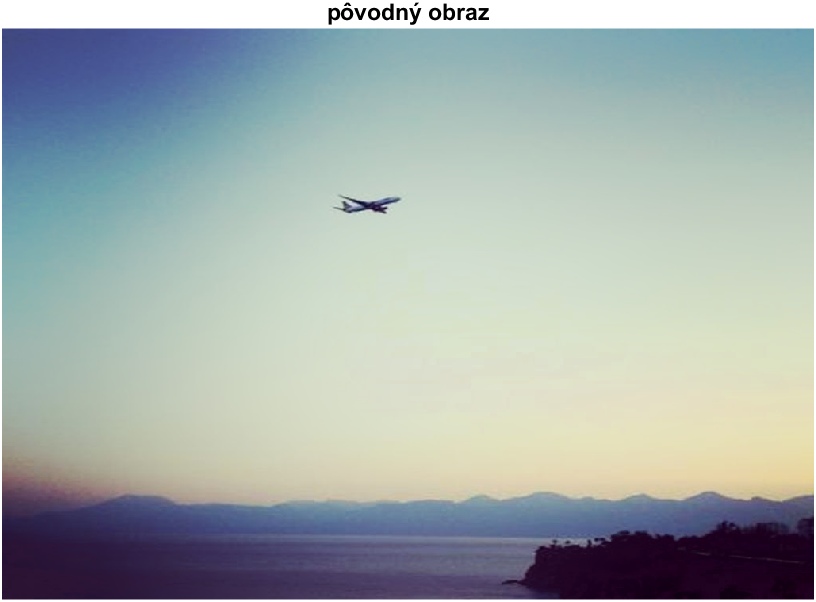
\includegraphics[width=.3\textwidth]{obrazky/canny/img.png}};
            \node (image2) [right of=image1] {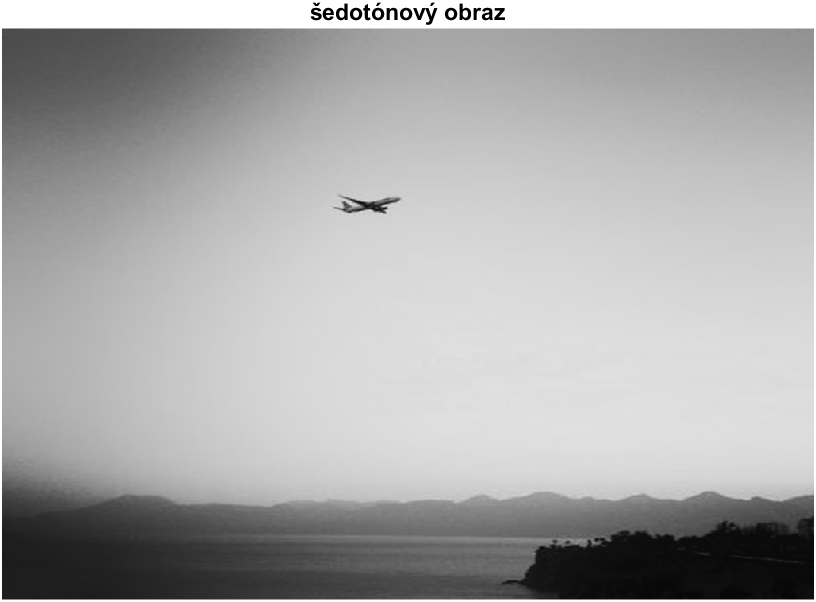
\includegraphics[width=.3\textwidth]{obrazky/canny/img_gray.png}};
            \node (image3) [right of=image2] {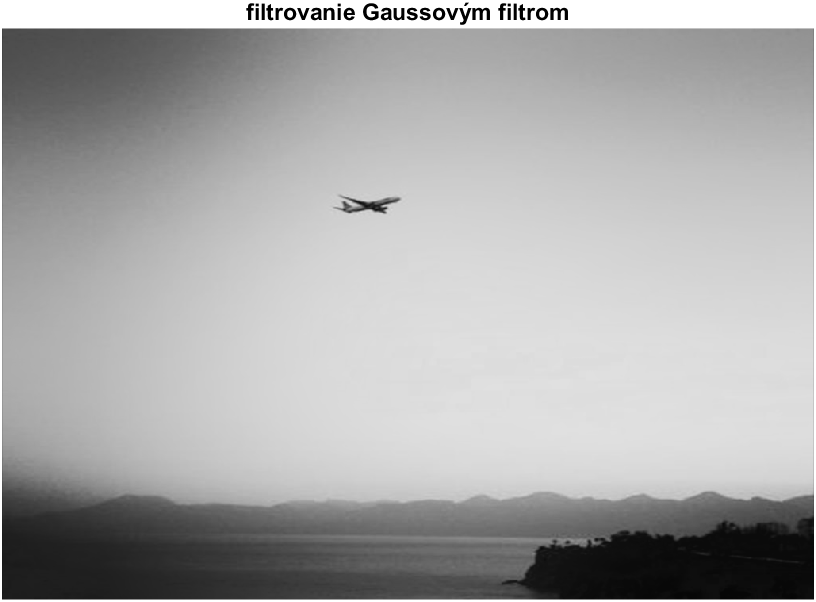
\includegraphics[width=.3\textwidth]{obrazky/canny/img_gauss.png}};
            \node (image4) [below of=image2] {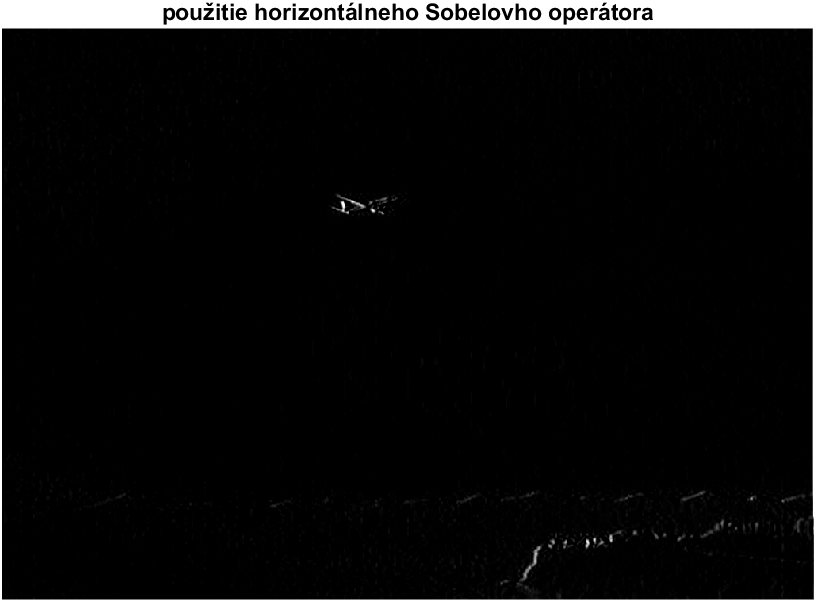
\includegraphics[width=.3\textwidth]{obrazky/canny/img_sobel_x.png}};
            \node (image5) [right of=image4] {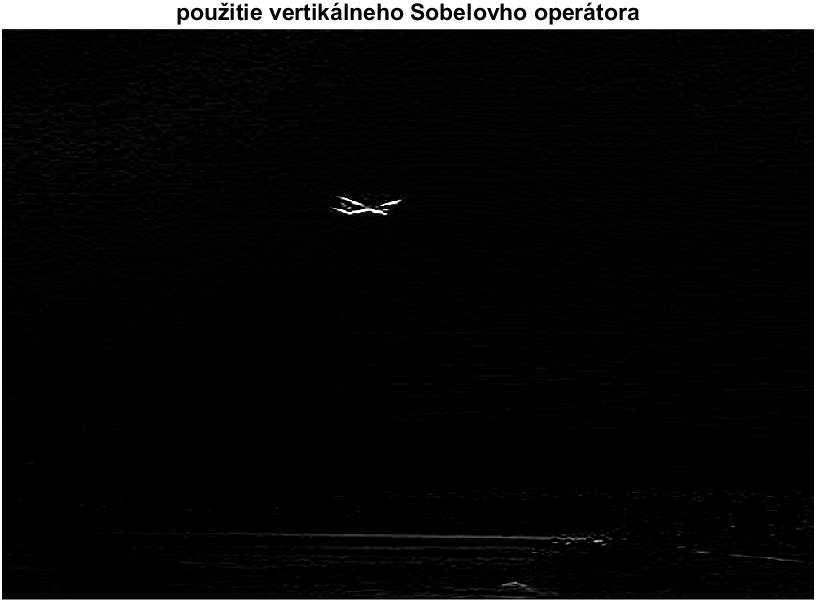
\includegraphics[width=.3\textwidth]{obrazky/canny/img_sobel_y.png}};
            \node (image6) [below of=image5] {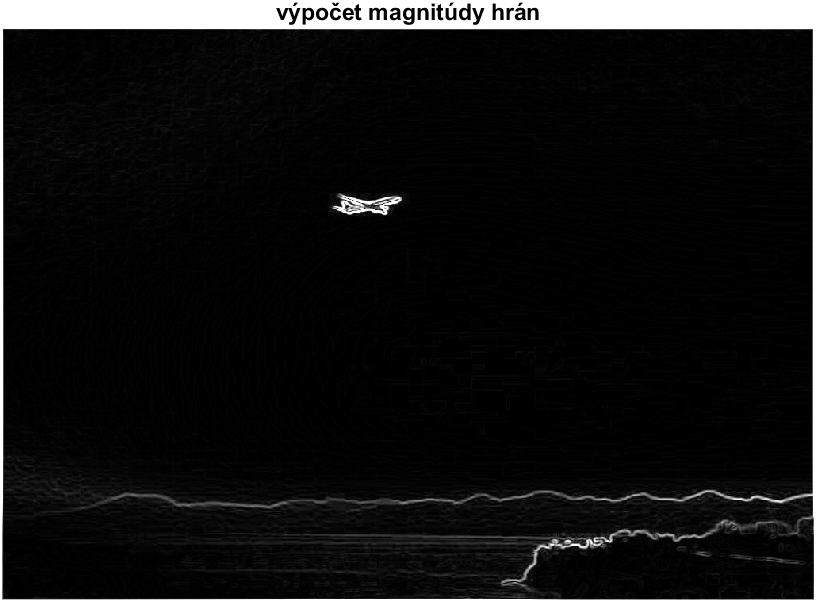
\includegraphics[width=.3\textwidth]{obrazky/canny/img_mag.png}};
            \node (image7) [left of=image6] {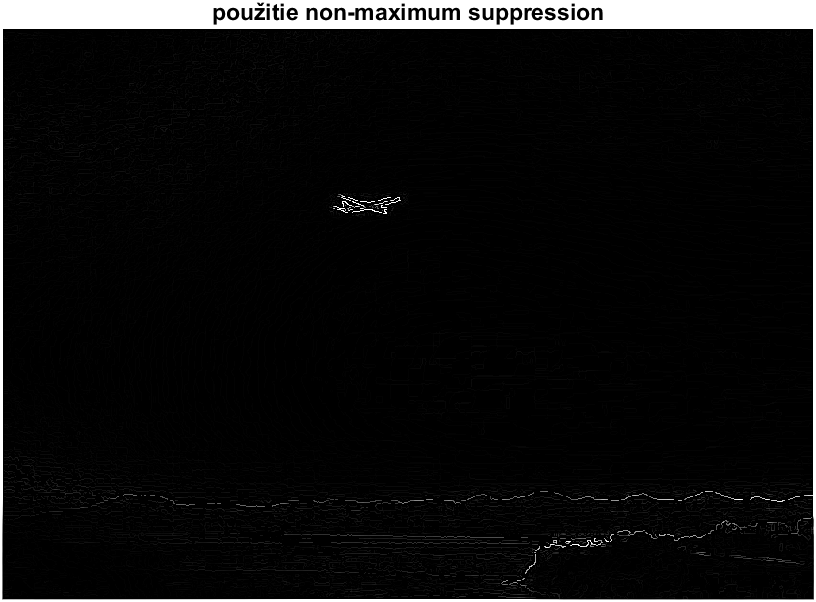
\includegraphics[width=.3\textwidth]{obrazky/canny/img_nms.png}};
            \node (image8) [left of=image7] {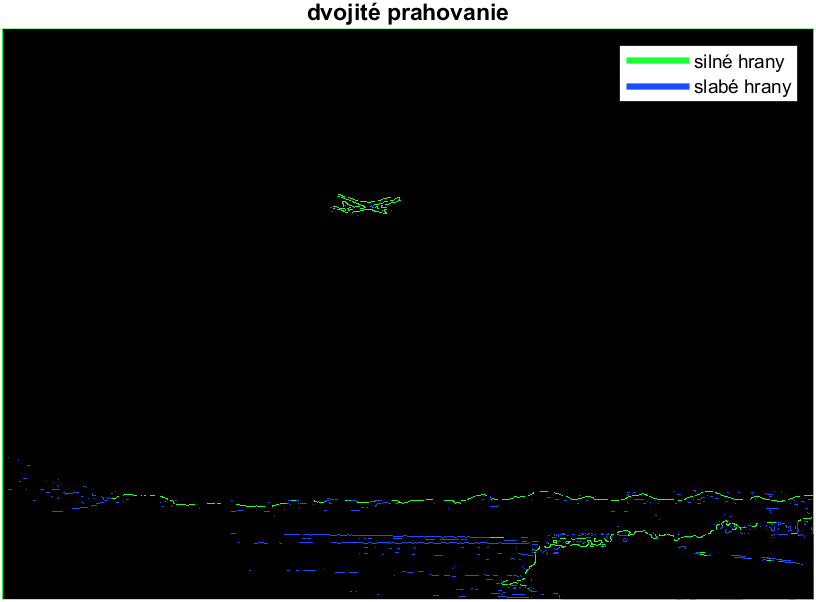
\includegraphics[width=.3\textwidth]{obrazky/canny/img_double_thresh.png}};
            \node (image9) [above of=image8] {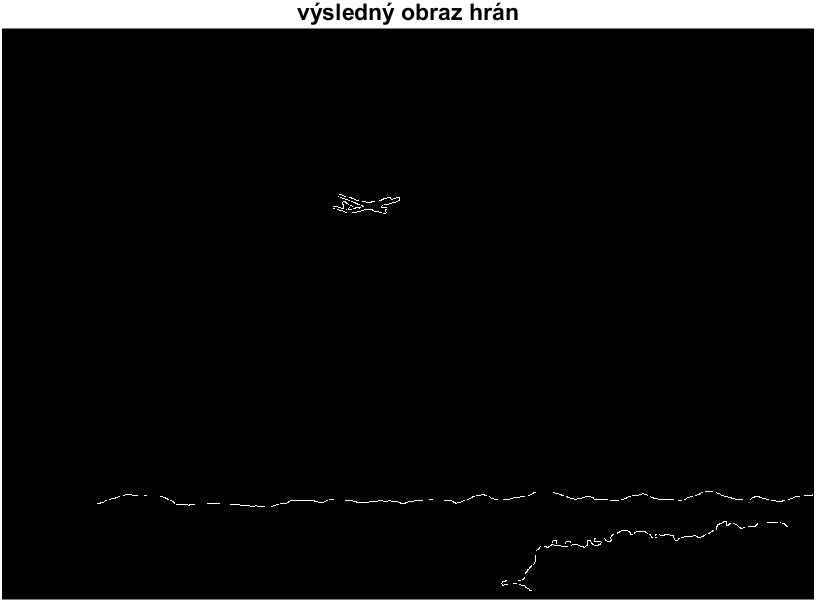
\includegraphics[width=.3\textwidth]{obrazky/canny/img_canny.png}};

            \draw[->] (image1) -- (image2) node[midway, above] {};
            \draw[->] (image2) -- (image3) node[midway, above] {};
            \draw[->] (image3) -- (image4) node[midway, above] {};
            \draw[->] (image3) -- (image5) node[midway, above] {};
            \draw[->] (image4) -- (image6) node[midway, above] {};
            \draw[->] (image5) -- (image6) node[midway, above] {};
            \draw[->] (image6) -- (image7) node[midway, above] {};
            \draw[->] (image7) -- (image8) node[midway, above] {};
            \draw[->] (image8) -- (image9) node[midway, above] {};
        \end{tikzpicture}
        \caption{Cannyho hranový detektor}
    \end{figure}

    Obraz hrán je možné ďalej spracovávať, napríklad morfologickýmy operáciami: otvorením odstrániť krátke nevýznamné hrany, zatvorením spojiť hrany blízko pri sebe.

    Vyhľadávaním uzavertých kontúr v obraze hrán je možné identifikovať potenciálne objekty v obraze.

    \subsection{Detekcia horizontu pomocou Houghovej transformácie}

        Pokiaľ časť obrazu obsahuje horizont, je vhodnejšie detekovať lietajúce objekty len na oblohe nad ním, aby sa predišlo falošným detekciám. Horizont je možné detekovať z obrazu hrán pomocou Houghovej transformácie, podľa práce. Vo výsledku Houghovej transformácie sa horizont prejaví ako najvýraznejšia čiara.


        \begin{figure}[H]
            \centering
            \begin{tikzpicture}[>=stealth, node distance=8cm]
                \node (image1) {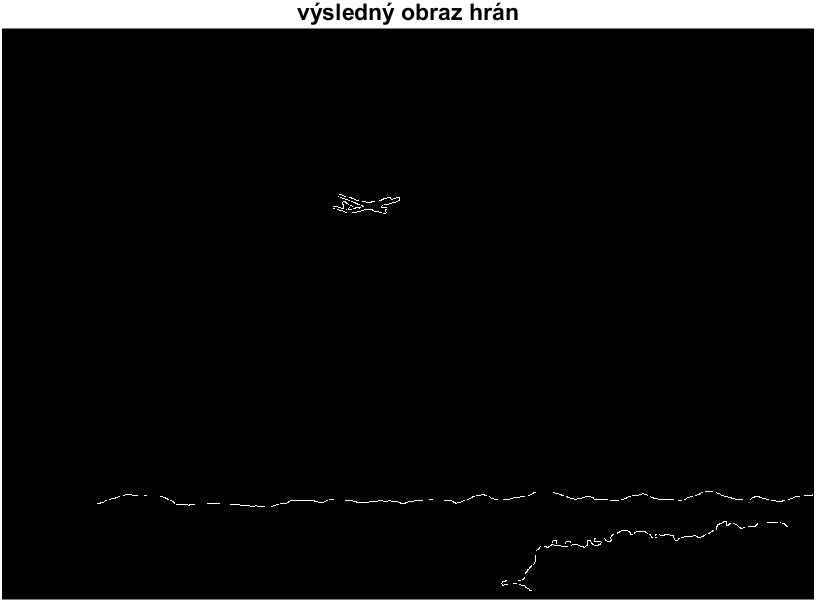
\includegraphics[width=.4\textwidth]{obrazky/canny/img_canny.png}};
                \node (image2) [below of=image1, yshift=2.5cm] {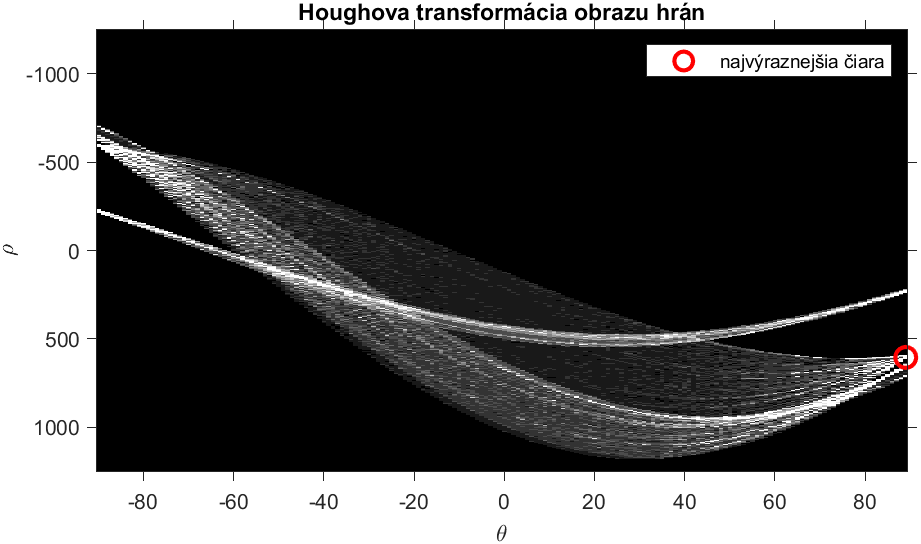
\includegraphics[width=.45\textwidth]{obrazky/canny/img_hough.png}};
                \node (image3) [right of=image2] {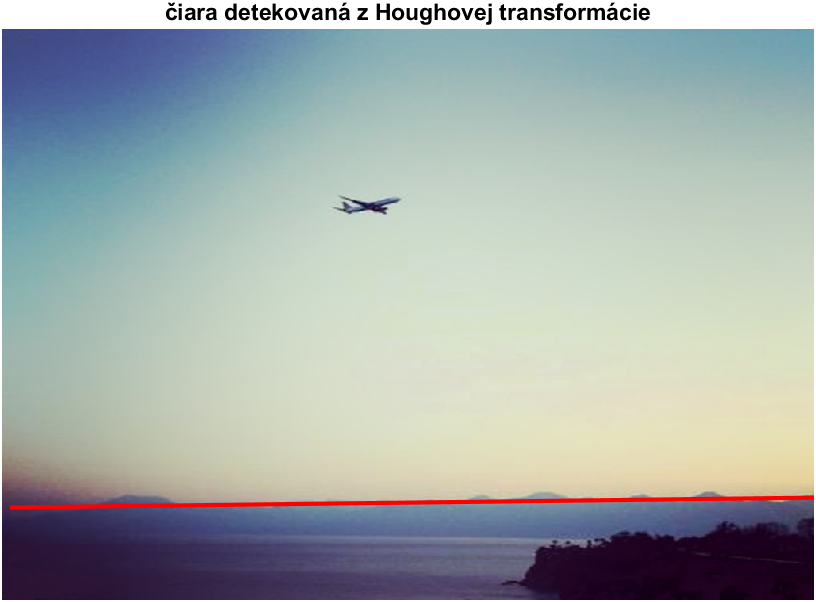
\includegraphics[width=.4\textwidth]{obrazky/canny/img_horizon.png}};

                \draw[->] (image1) -- (image2) node[midway, above] {};
                \draw[->] (image2) -- (image3) node[midway, above] {};
            \end{tikzpicture}
            \caption{Detekcia horizontu pomocou Houghovej transformácie}
        \end{figure}

\section{Detekcia pohybu}

    V prípade že je požadovaná detekcia pohybujúcich sa objektov, je možnosťou detekcie práve detekovaním ich pohybu. Jednou z jednoduchých metód detekcie pohybu sú rozdielové metódy, pri ktorých je vypočítavaný rozdielový snimok z viacerých snímkov zo sekvencie \(\{I_1, I_2, ..., I_n\}\). Rozdielový snímok môže byť:

    \begin{itemize}
        \item \textbf{jednostranný} - je najjednoduchší nenesie informáciu o smere pohybu, vyhodnocuje sa len v miestach kde \(I_1(x,y) > I_2(x,y)\).
        \[D(x,y) = \begin{cases}
            0 & I_1(x,y) - I_2(x,y) < \epsilon \\
            1 & I_1(x,y) - I_2(x,y) \geq \epsilon
        \end{cases}\]

        \item \textbf{obojstranný} - dostaneme ho upravením vzťahu pre jednostranný rozdielový snímok, použitím absolútnej hodnoty. Tým je dosiahnutá zameniteľnosť \(I_1(x,y)\) a \(I_2(x,y)\), vyhodnocuje sa teda na celom obraze. Neodstraňuje nedostatok informácie o smere pohybu, tá však nemusí byť nutnosťou.
        \[D(x,y) = \begin{cases}
            0 & |I_1(x,y) - I_2(x,y)| < \epsilon \\
            1 & |I_1(x,y) - I_2(x,y)| \geq \epsilon
        \end{cases}\]

        \item \textbf{kumulovaný} - je vytvorený váženým súčtom jedno alebo obojstranných rozdielových snímkov. Je teda možné priemerovať pohyb za určitý čas určením každej váhy \(\omega = 1/(N-1)\), alebo určiť rôznym snímkom rôznu váhu a získať tak informáciu o smere pohybu.
        \[D(x,y) = \sum_{i=1}^{N-1}\omega_i \cdot D_i(x,y)\]
    \end{itemize}

    Komplexnejšiou metódou detekcie pohybu je vytvorenie rozdielového snímku nie medzi nasledujúcimi snímkami, ale aktuálnym snímkom a vytvoreným modelom pozadia. Ten je možné zostaviť:

    \begin{itemize}
        \item ako jeden obraz pozadia bez objektov.
        \item ako priemerný snímok niekoľkých snímkov pozadia.
        \item ako dynamický model - iteratívnym aktualizovaním podľa aktuálneho snímku.
        %\begin{enumerate}
            %\item Výpočet rozdielového snímku \(D_1(x,y)\) z dvoch aktuálne najposlednejších snímkov sekvencie \(I_i(x,y)\) a \(I_{i-1}(x,y)\) .
        %\end{enumerate}
    \end{itemize}

    \begin{tikzpicture}[node distance=.7cm, auto]

        % Define block styles
        \tikzstyle{block} = [rectangle, draw, fill=white!20, text width=12em, text centered, sharp corners, minimum height=4em]
        \tikzstyle{line} = [draw, -latex']

        % Nodes
        \node [block] (start) {prejdi na ďalší snímok
        
        i \(\leftarrow\) i + 1};
        \node [block, below=of start] (calc_d1) {výpočet \(D_1(x,y)\) medzi \(I_i(x,y)\) a \(I_{i-1}(x,y)\)};
        \node [draw, diamond, aspect=4, below=of calc_d1] (check_d1) {vykazuje \(D_1(x,y)\) významný pohyb?};
        \node [block, below=of check_d1] (calc_d2) {vypočítaj \(D_2(x,y)\) medzi \(I_i(x,y)\) a \(B_i(x,y)\)};
        \node [draw, diamond, aspect=4, below=of calc_d2] (check_d2) {vykazuje \(D_2(x,y)\) významný pohyb?};
        \node [block, below=of check_d2] (calc_b) {vypočítaj \(B_{i+1}(x,y)\)};

        % Arrows
        \path [line] (start) -- (calc_d1);
        \path [line] (calc_d1) -- (check_d1);
        \path [line] (check_d1.west) -- ++(0,2.5) -- node [below = .3cm] {áno} (start.190);
        \path [line] (check_d1) -- node [near start] {nie} (calc_d2);
        \path [line] (calc_d2) -- (check_d2);
        \path [line] (check_d2.west) -- ++(-1,1) -- ++(0,7) -- node [near start] {áno} (start.170);
        \path [line] (check_d2) -- node [near start] {nie} (calc_b);
        \path [line] (calc_b.east) -- ++(3,1) -- ++(0,10) -- (start.east);

    \end{tikzpicture}